\section{Ponte H}
Os motores de corrente contínua trabalham nos dois sentidos de rotação quando invertidas suas polaridades. A ponte H é um circuito que tem a função de controlar esse sentido de rotação do motor a partir da inversão de sua polaridade. O exemplo a seguir, ilustra uma ponte H composta de quatro transístores que trabalham em pares nas diagonais. Basicamente, quando se aciona uma chave tem-se 12V e a outra chave-par leva o terra (0V) para o motor. A utilização de transístores NPN e PNP é aconselhável para evitar uma perda de tensão maior entre eles, dessa forma, a carga (motor) fica sempre ligado aos coletores dos transístores.     

\begin{figure}[H]
	\centering
	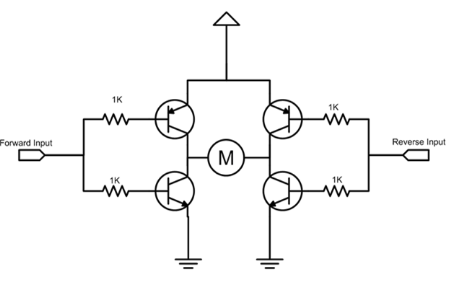
\includegraphics[width=5cm]{figuras/ponteH.png}
	\caption{Representação ponte H}
	\label{ponte H}
\end{figure}

Para o projeto Green House, será necessária a confecção de uma ponte H para controle da rotação do motor. Foi realizada uma simulação no Proteus®, afim de garantir a tensão de 12V para carga, a funcionalidade do circuito e demonstrada também a entrada do controlador de operações (representado pelos 3,3V):

\begin{figure}[H]
	\centering
	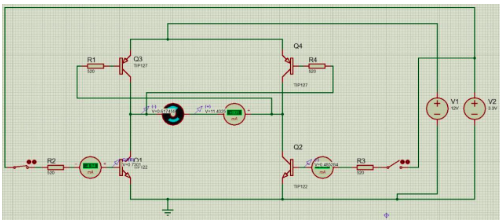
\includegraphics[width=7cm]{figuras/simulacaoPonteH.png}
	\caption{Simulação da ponte H com acionamento em Q1 e Q4. Fonte: Proteus*.}
	\label{simulação ponte H}
\end{figure}

\begin{figure}[H]
	\centering
	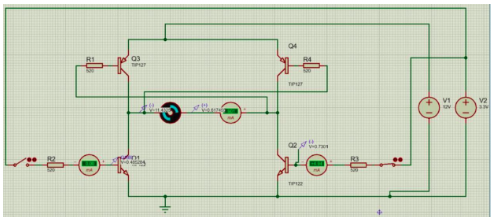
\includegraphics[width=7cm]{figuras/simulacaoPonteH2.png}
	\caption{Simulação da ponte H com acionamento em Q2 e Q3. Fonte: Proteus*.}
	\label{simulação ponte H 2}
\end{figure}

O microcontrolador que será utilizado é uma Raspberry que trabalha com 3,3V e tem limitação na corrente de 50mA, quando utilizadas todas as suas entradas. Assim, para que essa restrição seja limitada, no nó de conexão entre o transístor e o controlador, a corrente foi limitada a 0,005mA. Para isso ocorrer, é necessário o uso de resistências de 520$\Omega$, como demonstrado a seguir:

\begin{center}
	
$\frac{V_{cc} - V_{be}}{R}$ = $l_{b}$ \\
$\frac{3,3 - 0,7}{R}$ = 0,005\\
R = 520$\Omega$\\
$I_{ce}$ = 1000 $\Omega$ * 0,005 = 5 \textit{A}

\end{center}

Onde,
\begin{itemize}

	\item Ib = corrente que aciona o transistor;
	
	\item R = resistências que serão utilizadas para controle da corrente Ib;
	
	\item $I_{ce}$ = corrente disponível à carga;
	
	\item ${V_{cc} - V_{be}}$ = diferença de tensão entre o controlador e o transístor.
	
	\item A corrente $I_{ce}$ é multiplicada por 1000 devido ao transistor TIP. Sendo ela fornecida pela fonte que será construída mais adiante.
	
\end{itemize}

Para a construção dessa ponte H, serão necessários:
\begin{itemize}

\item 2 transístores Darlington TIP 120;
\item 2 transístores Darlington TIP 125;
\item 4 resistências de 520$\Omega$;
\item 1 placa furada;
\item 3 Borne Conector 2 vias - entradas PCI

\end{itemize}

\subsection{Confecção Ponte H}
A ponte H foi feita primeiramente em uma protoboard a fim de ser validada sua eficiência. Em seguida, o sistema foi transferido para a placa furada. O resistor utilizado apresentou mudança pois o item não estava disponível para a venda. Os resistores utilizados foram os 4 resistências de 560$\Omega$. Dessa forma:  

\begin{center}
	
	$\frac{3,3 - 0,7}{560}$ = $l_{b}$\\
	$l_{b}$ = 0,0046\textit{A}\\
	$I_{ce}$ = 1000 $\Omega$ * 0,0046 = 4,6 \textit{A}
	
\end{center}

\begin{itemize}

	\item $l_{b}$ = corrente que aciona o transistor;
	\item $I_{ce}$ = corrente disponível à carga.
	
\end{itemize}

O resultado final é mostrado a seguir:

\begin{figure}[H]
	\centering
	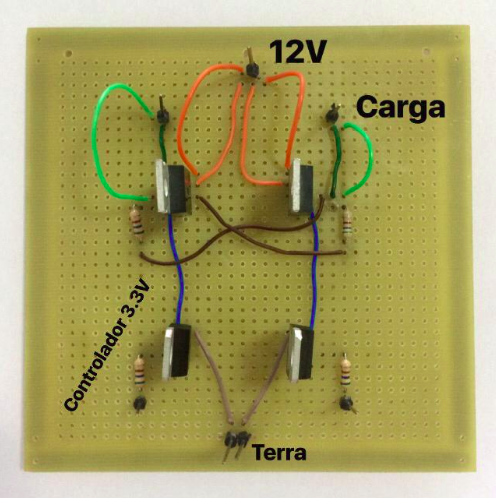
\includegraphics[width=13cm]{figuras/ponteHpronta.png}
	\caption{Ponte H confeccionada.}
	\label{ponte H pronta}
\end{figure}

Os integrantes que confeccionaram a placa tiveram dificuldades com a manipulação dos componentes, por não possuírem prática alguma com circuitos. Para posteriores trabalhos, é recomendado o uso de fios com bitolas maiores a fim de manter a segurança da ponte H.
